\documentclass[10pt,norsk,a4paper]{article}
\usepackage[utf8]{inputenc}
\usepackage[T1]{fontenc}
\usepackage[norsk]{babel}
\usepackage[cm]{fullpage}
\usepackage{color}
\usepackage{parskip,textcomp,amssymb,graphicx}
\usepackage{pdfpages}

\title{Generalforsamling\\
	Vår 2016\\
	Cybernetisk Selskab\\[.3cm]
	
\includegraphics[width=0.8\textwidth]{cyblogoa3.pdf}\\[-.5cm]}
\date{26. mai 2016}

\begin{document}
\maketitle{}
\tableofcontents{}

%\newpage
~\\

\section{Valg av møteleder}

\section{Valg av referent}

\section{Valg av protokollunderskrivere}

\section{Valg av tellekorps}

\section{Godkjenning av innkalling}

\section{Godkjenning av dagsorden}
Valg av Rekrutteringsansvarlig ble uteglemt i endelig dagsorden, og Hovedstyret spør derfor Generalforsamlingen om å godkjenne at vi har valg på Rekrutteringsansvarlig under valg av styremedlemmer i hovedstyret.

\newpage


\section{Semesterberetninger}
\subsection{Semesterberetning ved Leder}

Dette semesteret har ikke skilt seg markant fra tidligere semestre. Hovedtyngden av innsatsen ligger i fast drift av kafé og bar og denne varierer lite. Der vi derimot har sett en positiv økning er på arrangementer. Av større hendelser kan vi nevne at vi har fått gjenopptatt tradisjonen med faglig helg, vi har holdt en sikkelig feiring for Escapes 5års jubileum og vi har hatt fullt hus på et samarbeidsarrangement med innovasjonsutvalget hvor det var et foredrag med Jon von Tetzchner. Det har i flere semestre vært et uttalt mål å samarbeide bedre med andre foreninger og organisasjoner. Dette semesteret har vi startet opp samarbeid med både Innovasjonsutvalget og Erasmus Student Network, og spesielt samarbeidet med innovasjonsutvalget har vært veldig givende. Vi har også sett tendeser fra DEFI om ønske om samarbeid på et par arrangementer i Escape. Disse har vi dessverre ikke lyktes å kjøre som fullverdige samarbeidsarrangement, hovedsaklig på grunn av tidspunkter, men jeg er håper dette er noe vi kan jobbe videre med og med bedre planlegging er det gode muligheter for å åpne Escape enda mer opp for resten av foreningsmiljøet.

Alt i alt ser vi at vi har hatt en markant økning i aktiviteten. Dette semesteret har vært et godt steg opp fra forrige vårsemester og jeg håper virkelig denne veskten fortsetter og vi også neste semester klarer å legge lista der den har blitt lagt hittil i år. Jeg vil avslutte med å takke alle som har jobbet som frivillig dette semesteret. Ingenting av det vi har gjennomført ville vært mulig uten dere.\\

Jan Kristian Furulund,\\
Leder Cybernetisk Selskab\\
Vår 2016

%\newpage


\subsection{Semesterberetning ved Kjellermogul}

Blir lagt inn som vedlegg under Generalforsamlingen.

\newpage

\section{Regnskap}
Kasserer orientere om regnskap\\

%\newpage


\section{Revidert budsjett høst 2016}
Kasserer orientere om budsjett\\


%\newpage

\section{Kontingentfastsettelse}
Hovedstyret foreslår å holde medlemskontigenten på 30 kroner.\\

\section{Valg}

\begin{minipage}[t]{9cm}
\subsection{Hovedstyret}
Man velges inn i hovedstyret for ett år av gangen.
\subsubsection{Leder}

\subsubsection{Nestleder}

\subsubsection{Kjellermogul}

\subsubsection{Rekrutteringsansvarlig} 
Forutsetter at det blir godkjent i "Godkjenning av dagsorden"

\end{minipage}
\begin{minipage}[t]{9cm}
\subsection{Kjellerstyret}
Alle verv som er til valg i kjellerstyret, gjelder for ett semester av gangen.

\subsubsection{Barsjef}

\subsubsection{Innkjøpsansvarlig}

\subsubsection{Kafésjef}

\subsubsection{Teknisk ansvarlig}

\subsubsection{DJ-sjef}

\subsubsection{Utlånsansvarlig}

\end{minipage}

%\newpage
\newpage

\section{Vedtektsendringer}

\subsection{Vedtektsendring i §4:}
​§4 Revisjon punkt a) foreslås endret i sin helhet fra\\
"Leder i samarbeid med kasserer har som oppgave å engasjere en uavhengig tredjepart til å revidere regnskap for hvert hele år​"\\
til\\
"Hovedstyret skal utnevne minst to personer for å revidere årsregnskapet. Personene kan ikke ha vært medlemmer av økonomigruppa eller innehatt styreverv i perioden som revideres."

Formålet med dette er å åpne opp for at også interne/tidligere interne i foreningen kan bistå med revidering så fremt de ikke anses som inhabile. I tillegg ser vi det mer gunstig at det er en gruppe som forestår dette, og at det er hovedstyret som organ som utnevner revisorene.

I tillegg til dette er det ønskelig at det utarbeides en instruks for revisjon av regnskap som tar for seg nærmere detaljer, og at man gjennom denne instruksen prøver å få til mer fortløpende revidering enn en stor gjennomgang én gang årlig.

\subsection{Vedtektsendring i §5:}
Forandre §5e til "Hovedstyret kan med tre fjerdedels flertall oppnevne
hovedstyremedlemmer ved behov for etterfyl-
ling av alle verv foruten leder og kjellermogul. Den etterfylte sitter
frem til neste generalforsamling."

Grunn: §6e sier at vi ikke kan etterfylle kjellermogul i KS.

\subsection{Vedtektsendring i §7:}
Forandre §7f til: 
"Valg av styremedlemmer på Generalforsamling foregår skriftlig dersom det er to eller flere kandidater som stiller til vervet. Øvrige valg foregår ved håndsopprekning med mindre to av de stemmeberettigede ønsker skriftlig avstemming." 


\section{Æresmedlemskap}

\section{Utdeling av pins}
Arkivar deler ut pins\\

\section*{Vedlegg: Vedtekter}

\newpage

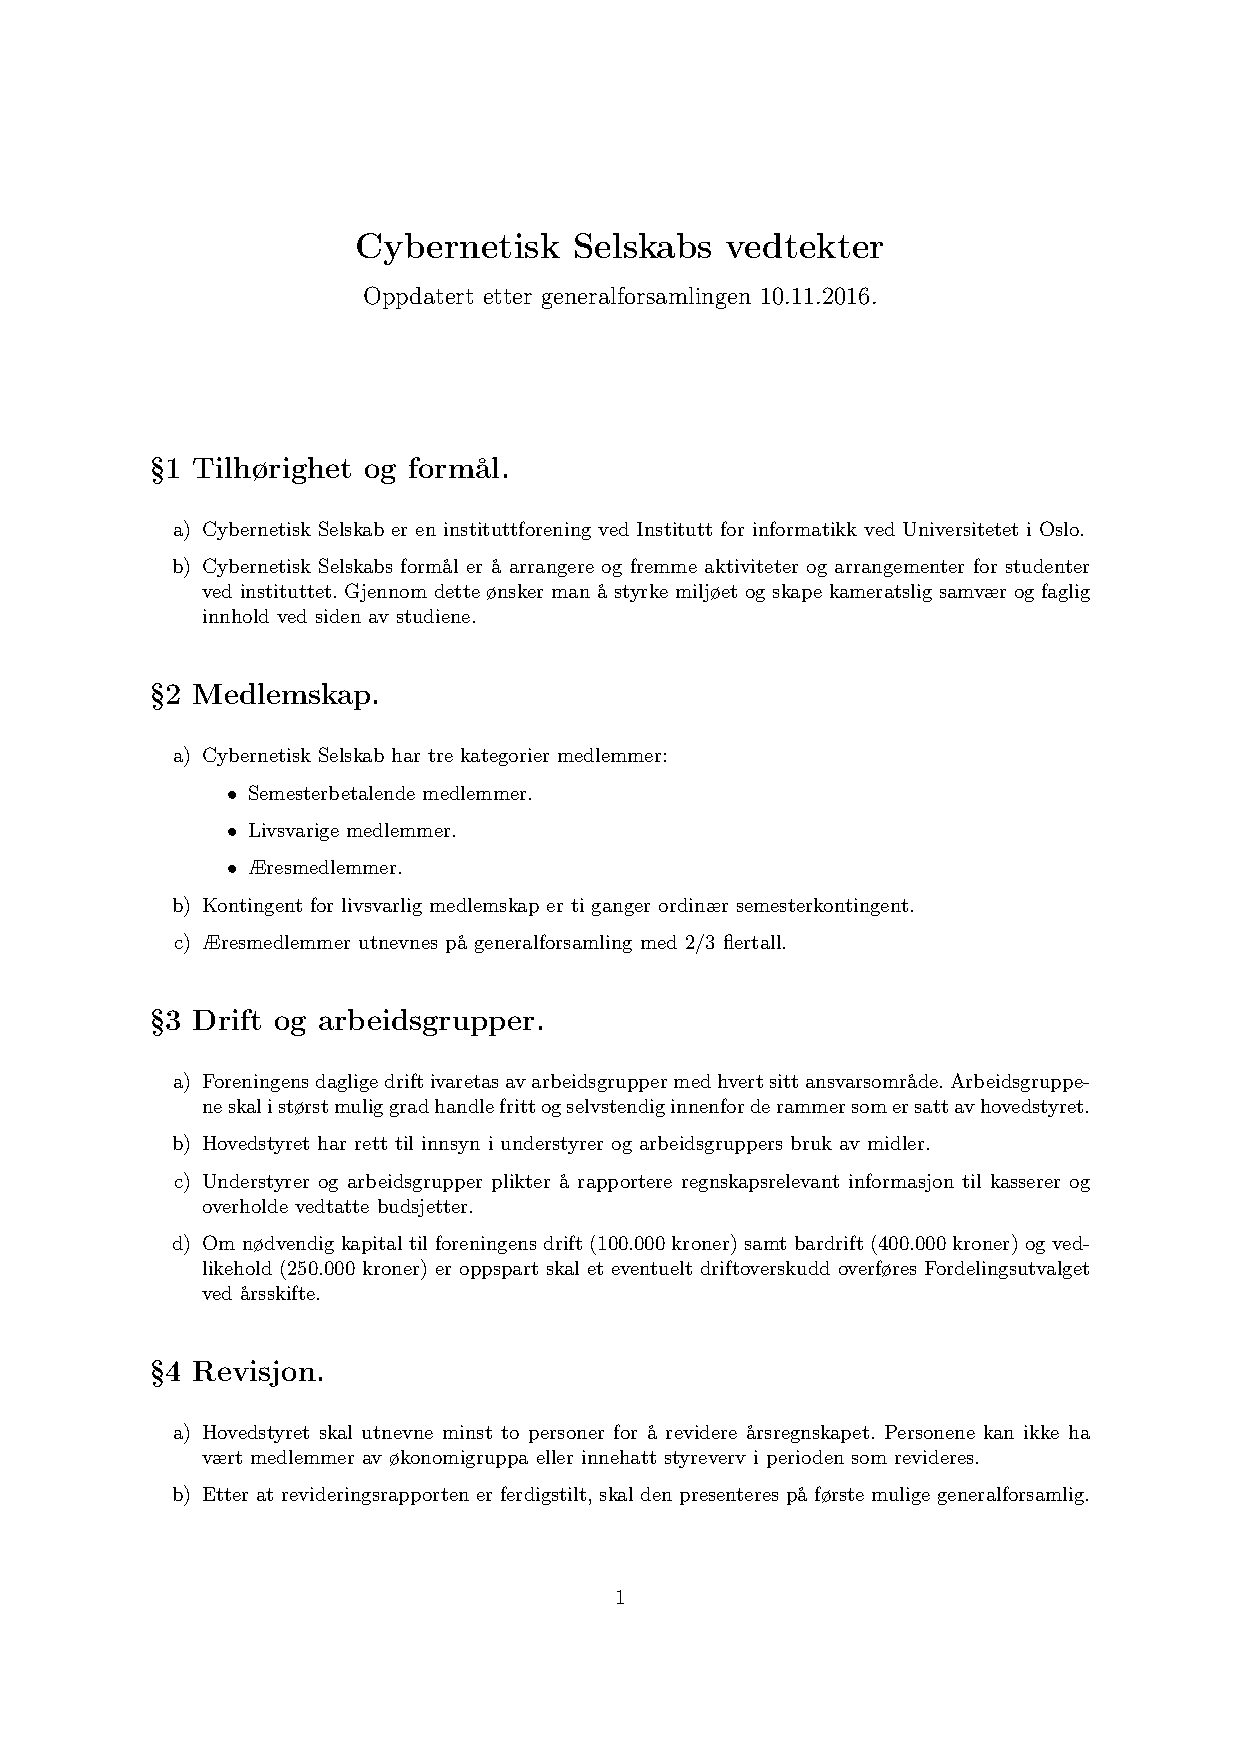
\includepdf[pages=-]{cyb_vedtekter.pdf}
\end{document}
